\documentclass[a4paper, oneside]{Thesis}

\usepackage{wrapfig}
\usepackage{lscape} % FIXED
\usepackage{rotating}
\usepackage{graphicx}
\usepackage{caption}
\usepackage{amsmath}
\usepackage{xcolor}
\usepackage[most]{tcolorbox}
\usepackage{amssymb}
\usepackage{array}
\usepackage{float}
\usepackage{placeins}
\usepackage{stackengine}
\usepackage{url}
\usepackage{numprint}
\usepackage{algorithm}
\usepackage{algpseudocode}
\usepackage{booktabs}
\usepackage{siunitx}
\usepackage{subcaption} % FIXED
\usepackage{setspace}   % FIXED

\usepackage{natbib}
\usepackage{hyperref}   % MOVED LAST

\nprounddigits{3}
\newcolumntype{P}[1]{>{\centering\arraybackslash}p{#1}}
\newcolumntype{M}[1]{>{\centering\arraybackslash}m{#1}}

\setstackEOL{\#}
\setstackgap{L}{10pt}
\usepackage{eso-pic}

\newcommand{\AddCertSignatureLine}{%
  \AddToShipoutPictureFG*{%
    \AtTextUpperLeft{%
      \raisebox{-0.36\textheight}[0pt][0pt]{%
        \makebox[\textwidth]{%
          \begin{minipage}{\textwidth}
            \centering
            \rule{7cm}{0.4pt}\\[-0.15em]
            \small Supervisor's Signature
          \end{minipage}
        }%
      }%
    }%
  }%
}

\graphicspath{{Pictures/}}
\usepackage{natbib}

\hypersetup{urlcolor=black, colorlinks=false}

%------------------------------------------------------------------------
%  THESIS METADATA  — update these fields as required
%------------------------------------------------------------------------
\thesistitle{Pricing ESG Changes in the CAPM: An Empirical Analysis of Return Predictability and Beta Amplification}
\supervisor{Professor Ajay Kumar Mishra}
\degree{B.Tech(Hons.) and M.Tech(Dual Degree)}
\degreemajor{Chemical Engineering and Financial Engineering}
\authors{Shamik Bhattacharjee}
\rollno{22CH3FP11}
\university{Indian Institute of Technology Kharagpur}
\newcommand{\primarydept}{Department of Chemical Engineering}
\newcommand{\secondarydept}{Vinod Gupta School of Management}
\department{\primarydept}
\unisite{http://www.iitkgp.ac.in}
\depsite{http://www.iitkgp.ac.in}
\placeshrt{Kharagpur}
\placelng{Kharagpur - 721302, India}
\datesub{}
\datesig{}
\semsub{Spring Semester, 2025-26}
\coursecd{Bachelor Thesis Project}

\title{\ttitle}

\begin{document}

\frontmatter
\setstretch{1.6}

\fancyhead{}
\rhead{\thepage}
\lhead{}

\newcommand{\HRule}{\rule{\linewidth}{0.5mm}}

\hypersetup{pdftitle={\ttitle}}
\hypersetup{pdfsubject=\subjectname}
\hypersetup{pdfauthor=\authornames}
\hypersetup{pdfkeywords=\keywordnames}

%----------------------------------------------------
%  TITLE PAGE
%----------------------------------------------------
\maketitle
\clearpage

%----------------------------------------------------
%  DECLARATION
%----------------------------------------------------
\Declaration

%----------------------------------------------------
%  CERTIFICATE
%----------------------------------------------------
\addtotoc{Certificate}
\department{\secondarydept}
\certificate{\addtocontents{toc}{}}
\department{\primarydept}
\clearpage

\setstretch{1.3}

%----------------------------------------------------
%  ACKNOWLEDGEMENTS
%----------------------------------------------------
\acknowledgements{

I would like to express my deepest gratitude to my supervisor,
Prof.\ Dr.\ Ajay Kumar Mishra for his guidance, encouragement,
and steady intellectual support throughout this project. His ability
to connect methodological rigour with practical financial insight
shaped this thesis in ways I could not have managed independently.


Finally, I thank my parents for their unwavering support, and my
friends for their encouragement at every stage of this project.

}
\clearpage

%----------------------------------------------------
%  ABSTRACT
%----------------------------------------------------
\addtotoc{Abstract}
\abstract{\addtocontents{toc}{}
This thesis investigates whether changes in environmental, social, and governance (ESG) characteristics, rather than their static levels, are priced in equity markets. Using a panel of S\&P 500 firms over the period 2015–2024, the study constructs a time-varying ESG measure to capture within-firm dynamics. The analysis is conducted within a CAPM-based framework augmented with ESG variables to examine both return predictability and systematic risk.

The results show that ESG levels do not command a robust cross-sectional premium, indicating that static sustainability characteristics are largely incorporated into market prices. In contrast, improvements in ESG are associated with positive contemporaneous returns and exhibit predictive power for future returns, even after controlling for standard risk factors. This provides evidence of an ESG momentum effect consistent with gradual information diffusion and institutional rebalancing.

A key finding is that ESG improvements increase market beta, revealing a \textit{Beta Amplification Paradox} in which firms undergoing sustainability transitions experience higher exposure to systematic risk. Additional analysis shows that individual ESG components are not priced in isolation, while sector-level results indicate that effects are concentrated in industries where ESG considerations are economically material. Overall, the findings highlight ESG as a dynamic and state-dependent pricing factor with implications for asset pricing and portfolio construction.



}
\clearpage

%----------------------------------------------------
%  TABLE OF CONTENTS
%----------------------------------------------------
\pagestyle{fancy}

\tableofcontents
\clearpage

%\setstretch{1.5}

%----------------------------------------------------
%  LIST OF FIGURES
%----------------------------------------------------
%\lhead{\emph{List of Figures}}
%\listoffigures
%\clearpage

%----------------------------------------------------
%  LIST OF TABLES
%----------------------------------------------------
%\lhead{\emph{List of Tables}}
%\listoftables
%\clearpage

%----------------------------------------------------
%  ABBREVIATIONS
%----------------------------------------------------
%\lhead{\emph{Abbreviations}}
\listofsymbols{ll}{
  \textbf{CAPM}  & Capital Asset Pricing Model \\
  \textbf{CMA}   & Conservative Minus Aggressive (Fama-French factor) \\
  \textbf{ESG}   & Environmental, Social, and Governance \\
  \textbf{FE}    & Fixed Effects \\
  \textbf{FF5}   & Fama-French Five-Factor Model \\
  \textbf{FM}    & Fama-MacBeth \\
  \textbf{GICS}  & Global Industry Classification Standard \\
  \textbf{HC3}   & Heteroskedasticity-Consistent (Davidson-MacKinnon) \\
  \textbf{HML}   & High Minus Low (book-to-market factor) \\
  \textbf{HML$_{\text{ESG}}$} & High-Minus-Low ESG portfolio \\
  \textbf{NW}    & Newey-West \\
  \textbf{OLS}   & Ordinary Least Squares \\
  \textbf{OU}    & Ornstein-Uhlenbeck \\
  \textbf{RMW}   & Robust Minus Weak (profitability factor) \\
  \textbf{SASB}  & Sustainability Accounting Standards Board \\
  \textbf{SMB}   & Small Minus Big (size factor) \\
}

%========================================================
%  MAIN MATTER
%========================================================
\mainmatter
\pagestyle{fancy}

%========================================================
% CHAPTER 1: INTRODUCTION
%========================================================
\chapter{Introduction}
\label{chap:introduction}

\section{Motivation}

The dominant question in ESG investing has long been whether being sustainable pays. Decades of empirical work have tried to establish whether firms with high ESG scores earn superior risk-adjusted returns --- the so-called ``greenium'' --- yet the evidence remains decidedly mixed \citep{friede2015esg, berg2022aggregate}. This thesis argues that the question itself is misconceived. The relevant question is not whether being green pays, but whether \emph{becoming} green pays.

The distinction matters for a simple reason: if high ESG scores are already embedded in prices through investor demand, there is no return premium to harvesting a static level. The premium, if it exists, must be located in the \emph{transition} --- in the information conveyed by an ESG improvement and the market reaction to it. This paper shifts the empirical lens from ESG state to ESG change, and finds a consistent, statistically robust set of pricing effects that static ESG level cannot generate.

The Capital Asset Pricing Model provides the pricing framework. Standard CAPM and its Fama-French extensions treat systematic risk as fixed, yet a firm undergoing an ESG transition is not a static entity: it is restructuring operations, reallocating capital expenditure, and attracting or shedding a new investor base. All of these forces alter the firm's sensitivity to market-wide shocks. The CAPM, as standardly estimated, has no mechanism for capturing this. This thesis builds one.

\section{What This Thesis Does}

Using a time varying panel of 479 S\&P 500 firms over February 2015 to December 2024 (56,656 firm-month observations), this thesis augments the CAPM with time-varying ESG change ($\Delta$ESG) and tests four empirically distinct claims.

First, ESG level carries no reliable cross-sectional risk premium. The Fama-MacBeth test yields $t = 1.086$ ($p = 0.280$): static ESG is already priced in and generates no exploitable spread. By contrast, within-firm ESG level variation is significantly priced ($t = 3.691$, $p = 0.0002$) in the fixed-effects panel, confirming that it is the \emph{movement} relative to a firm's own baseline that matters.

Second, ESG improvements are priced contemporaneously. Model M6 shows that month-over-month ESG change earns a significant positive return premium ($\hat{\beta} = 0.0203$, $t = 2.394$, $p = 0.017$), reflecting rapid market incorporation of the information content in rating revisions.

Third, lagged ESG improvements predict next-month returns even after Fama-French five-factor controls ($\hat{\gamma} = 0.0243$, $t = 3.14$, $p = 0.0017$). This ESG momentum channel is consistent with gradual institutional portfolio rebalancing and establishes $\Delta$ESG as a viable predictive factor.

Fourth --- and most originally --- ESG improvements \emph{amplify} market beta rather than dampening it ($\hat{\beta}_{int} = 0.5304$, $t = 2.814$, $p = 0.005$). This ``Beta Amplification Paradox'' directly contradicts the conventional narrative that sustainable firms are lower-risk. Firms in active ESG transition attract correlated institutional flows and face heightened operational uncertainty, both of which increase their co-movement with the market during the transition period.

\section{Contributions}

This thesis makes three contributions. First, it reframes the ESG-return debate around dynamics rather than levels, resolving the otherwise contradictory evidence on static ESG pricing. Second, it documents the Beta Amplification Paradox --- the empirical finding that ESG improvements temporarily increase systematic risk --- which has direct implications for how ESG is used in risk models and portfolio construction. Third, it demonstrates that individual E, S, and G pillars carry no return signal when considered in isolation: it is the aggregate composite change that the market prices, consistent with ESG as a holistic ``monolith'' rating rather than a sum of independent characteristics.

\section{Outline}

Chapter~\ref{chap:literature} reviews the literature on CAPM extensions, ESG pricing, and ESG dynamics. Chapter~\ref{chap:framework} presents the model framework, data construction, and methodology --- including the diagnostic pipeline that justifies fixed effects over random effects and clustered standard errors. Chapter~\ref{chap:results} reports the four core results. Chapter~\ref{chap:discussion} discusses mechanisms, limitations, and conclusions. Appendices contain full regression tables, portfolio sorts, and the Kalman-OU technical derivations.
%========================================================
% CHAPTER 2: LITERATURE REVIEW
%========================================================
\chapter{Literature Review}
\label{chap:literature}

\section{CAPM and Time-Varying Risk}

The Capital Asset Pricing Model, independently developed by \citet{sharpe1964capital} and \citet{lintner1965valuation}, establishes that in equilibrium, the expected excess return of an asset is proportional to its covariance with the market portfolio. Despite well-documented empirical anomalies, the CAPM remains the dominant framework for connecting risk and return in both research and practice. The Fama-French three-factor model \citep{fama1993common} and its five-factor extension \citep{fama2015five} added size (SMB), value (HML), profitability (RMW), and investment (CMA) factors to better describe the cross-section of returns. These extensions treat beta as fixed over time, an assumption that has been questioned by a growing literature on time-varying risk. \citet{harvey1989time} and \citet{ferson1996measuring} demonstrate that conditional betas fluctuate with the business cycle, while \citet{ang2007capm} show that static CAPM fails precisely during periods of high market stress. Any firm attribute that systematically alters a firm's risk profile --- including active ESG transition --- should, in principle, affect its time-varying beta.

\section{ESG and Equity Returns: The Static Impasse}

The ESG-return literature is characterised by heterogeneity. Early work by \citet{renneboog2008socially} and \citet{hong2009price} suggested that socially responsible investing imposes a financial cost, as ``sin stocks'' excluded from ESG portfolios earn superior returns. More recent meta-analytic evidence \citep{friede2015esg} finds that the majority of studies report a non-negative ESG-return relationship. \citet{edmans2011does} documents a positive long-run return to high employee satisfaction firms. \citet{khan2016corporate} find that only \emph{material} ESG characteristics predict returns, while immaterial ESG scores do not --- an early indication that the blanket aggregate score conflates relevant and irrelevant information.

The aggregate confusion is further compounded by ESG rating disagreement. \citet{berg2022aggregate} document substantial divergence across major ESG rating providers for the same firms, which mechanically reduces the statistical power of any cross-sectional ESG-return test. When ratings disagree, level-based cross-sectional tests are noisy by construction.

\citet{pastor2021sustainable} provide a theoretical reconciliation: ESG-rated firms earn lower expected returns in equilibrium because ESG-motivated investors bid up their prices, yet they show higher realised returns during periods of increasing investor ESG taste due to re-rating demand. This framework implies that the return to ESG is inherently dynamic --- driven by changes in investor preferences and ESG score revisions --- rather than by a static level premium. This thesis builds on precisely this insight.

\section{ESG Dynamics, Momentum, and Materiality}

The treatment of ESG as a dynamic variable is a recent development. \citet{giese2019foundations} document that ESG score revisions by major rating agencies are associated with abnormal returns around the event window, consistent with a price discovery channel. \citet{serafeim2020public} show that firms experiencing positive ESG momentum subsequently outperform those with flat or declining scores. \citet{lioui2021esg} argue that ESG momentum proxies for an omitted information channel: rating agencies incorporate information about future operational risk that is only gradually impounded in prices.

The ESG momentum channel connects naturally to the broader momentum literature. \citet{jegadeesh1993returns} document that past-winner stocks outperform past-losers over intermediate horizons. The delayed information diffusion mechanism of \citet{hong1999unified} --- investor underreaction to new information --- applies directly to ESG: if ESG changes convey information that institutional funds incorporate only gradually due to mandate constraints and rebalancing costs, lagged ESG changes should predict future returns.

The materiality dimension of ESG is formalised in the Sustainability Accounting Standards Board (SASB) framework, which identifies industry-specific ESG issues as financially material or immaterial based on their expected impact on enterprise value. \citet{khan2016corporate} provide the key empirical validation: only SASB-material ESG characteristics predict future returns, while immaterial ones carry no signal. This finding motivates the sector-level heterogeneity analysis in Chapter~\ref{chap:results}: ESG improvements in capital-intensive sectors such as Materials and Industrials represent genuine mitigation of regulatory and environmental risk and should be priced; ESG improvements in Information Technology may be perceived as immaterial CSR activity and should not.

Finally, the ``transition risk'' concept \citep{christophersen2022transition} describes the financial risks borne by firms during the process of improving their ESG profile: capital expenditure on new infrastructure, operational restructuring, and reputational uncertainty during the transition. This literature motivates our Beta Amplification Paradox hypothesis: firms actively improving ESG face elevated operational uncertainty precisely because they are in transition, which may temporarily increase their systematic risk loading rather than reduce it.
%========================================================
% CHAPTER 3: MODEL FRAMEWORK, DATA, AND METHODOLOGY
%========================================================
\chapter{Model Framework, Data, and Methodology}
\label{chap:framework}

%----------------------------------------------------
\section{Model Framework}
%----------------------------------------------------

\subsection{Baseline CAPM (M1)}

The standard CAPM frames the expected excess return of firm $i$ as:
\begin{equation}
  R_{i,t} - R_{f,t} \;=\; \alpha_i \;+\; \beta_i\bigl(R_{m,t} - R_{f,t}\bigr) \;+\; \varepsilon_{i,t}
  \label{eq:capm}
\end{equation}
where $R_{f,t}$ is the risk-free rate and $R_{m,t}$ is the value-weighted market return. This serves as the M1 benchmark.

\subsection{ESG Level (M2, M2C)}

Model M2 adds the time-varying normalised ESG level $\mathrm{ESG}_{i,t}$ as a return predictor:
\begin{equation}
  R_{i,t} - R_{f,t} \;=\; \alpha_i \;+\; \beta_1\bigl(R_{m,t}-R_{f,t}\bigr) \;+\; \beta_2\,\mathrm{ESG}_{i,t} \;+\; \varepsilon_{i,t}
  \label{eq:m2}
\end{equation}
With entity fixed effects and a time-varying panel, $\beta_2$ is identified purely from \emph{within-firm} ESG variation --- not cross-sectional differences. Model M2C adds a mean-centred interaction $\mathrm{ESG}_{i,t}^c \times (R_{m,t}-R_{f,t})$ to test whether the ESG \emph{level} modulates market beta. The insignificance of this interaction (H6: $t=1.442$, $p=0.149$) provides the null against which the $\Delta$ESG interaction in M6 is contrasted.

\subsection{ESG Change: The Core Model (M6)}

Model M6 replaces the ESG level with its mean-centred month-over-month change $\Delta\mathrm{ESG}_{i,t}^c$ and includes the interaction with the market factor:
\begin{equation}
  R_{i,t} - R_{f,t} \;=\; \alpha_i \;+\; \beta_1\bigl(R_{m,t}-R_{f,t}\bigr) \;+\; \beta_2\,\Delta\mathrm{ESG}_{i,t}^c \;+\; \beta_3\,\Delta\mathrm{ESG}_{i,t}^c\times\bigl(R_{m,t}-R_{f,t}\bigr) \;+\; \varepsilon_{i,t}
  \label{eq:m6}
\end{equation}
Mean-centring $\Delta\mathrm{ESG}$ before forming the interaction term resolves the multicollinearity inherent in interaction models, confirmed by a max VIF of 1.075 (see Section~\ref{sec:diagnostics}). $\beta_2$ tests whether ESG improvements are contemporaneously priced (H3). $\beta_3$ tests whether ESG change modulates systematic risk (H5) --- the Beta Amplification Paradox.

\subsection{ESG Momentum: Predictive Specification (P1--P3)}

Three specifications test whether lagged $\Delta\mathrm{ESG}$ predicts next-month returns:
\begin{equation}
  R_{i,t} - R_{f,t} \;=\; \alpha_i \;+\; \sum_{k}\gamma_k f_{k,t} \;+\; \gamma_6\,\Delta\mathrm{ESG}_{i,t-1}^c \;+\; \varepsilon_{i,t}
  \label{eq:momentum}
\end{equation}
P1 includes only entity and year fixed effects; P2 adds Mkt-RF; P3 adds the full Fama-French five-factor set. A significant $\gamma_6$ in P3 (H4) establishes ESG momentum as an independent predictive channel net of all standard risk factors.

\subsection{Component-Level Decomposition}

To test whether the aggregate ESG signal or its sub-components drive results, we re-estimate M6 and P3 replacing $\Delta\mathrm{ESG}^c$ with $\Delta E^c$, $\Delta S^c$, and $\Delta G^c$ separately. If the market prices the holistic rating rather than its individual dimensions, component-level regressions should yield insignificant coefficients even when the aggregate is significant.

\subsection{Economic Intuition}

Each coefficient has a clear economic story. $\beta_2$ reflects the information channel: an ESG revision signals changes in regulatory exposure, governance quality, or operational sustainability that the market prices rapidly. $\beta_3$ tests whether firms in ESG transition decouple from or amplify market co-movement. $\gamma_6$ tests whether ESG information is fully absorbed on impact or whether gradual institutional rebalancing generates persistent predictability. The Fama-MacBeth cross-sectional tests (H2) separately ask whether the level of ESG commands a cross-sectional risk premium independent of within-firm dynamics.

%----------------------------------------------------
\section{Data}
%----------------------------------------------------

\subsection{Sample and Variables}

The sample consists of 479 S\&P 500 constituent firms with continuous Sustainalytics ESG coverage over February 2015 to December 2024, yielding \textbf{56,656 firm-month observations}. Monthly total returns are from CRSP; Fama-French five-factor returns and the risk-free rate are from Kenneth French's data library. Sectors follow the eleven-sector GICS classification.

Sustainalytics scores are risk measures: higher raw scores indicate greater unmanaged ESG exposure. All scores are normalised to $[0,1]$ with direction inverted so that higher $\mathrm{ESG}_{i,t}$ denotes lower ESG risk (better ESG). The panel mean is 0.586 (SD $\approx$ 0.19). Industrials and Financials each contribute 74 firms; Consumer Discretionary contributes 46.

\begin{figure}[H]
  \centering
  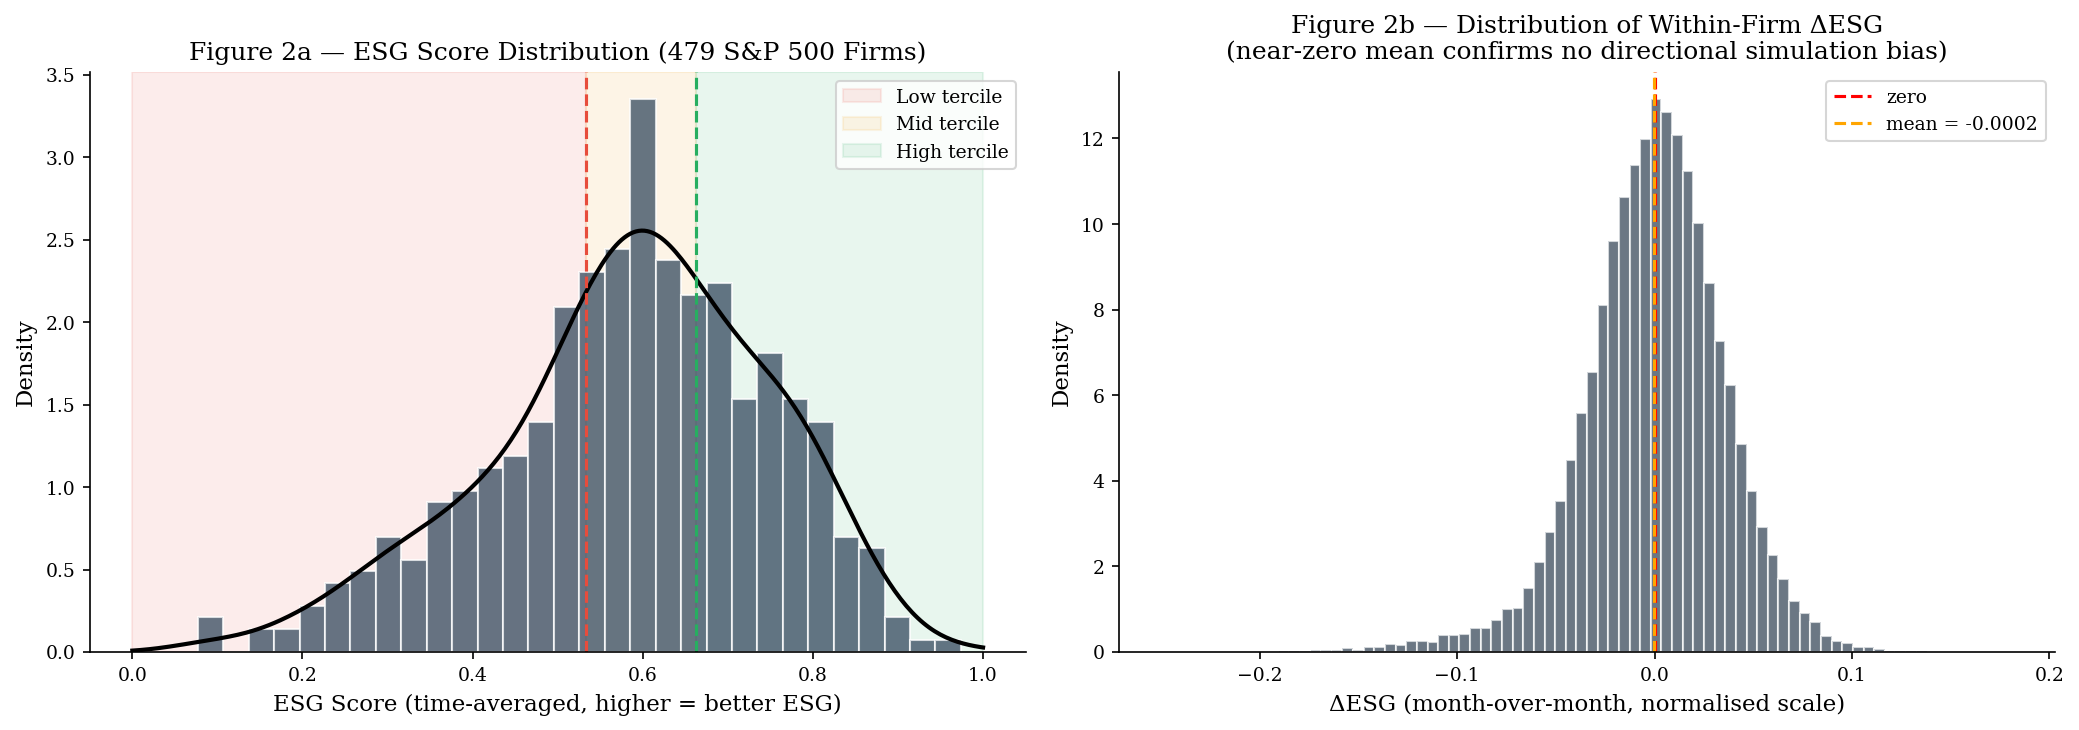
\includegraphics[width=\textwidth]{../Pictures/fig2_esg_dynamics.png}
  \caption{\textbf{Figure 2 --- ESG score distribution vs. $\Delta$ESG distribution }
  Diagnostics for Simulated ESG Dynamics.}
  Diagnostic views of the interpolated ESG panel, including the distribution of within-firm $\Delta\mathrm{ESG}_{i,t}$ and sector-level heterogeneity in ESG evolution. The near-symmetry around zero indicates no directional interpolation bias.}
  \label{fig:esg_distribution}
\end{figure}



\subsection{Time-Varying ESG Panel via Stochastic Interpolation}
\label{sec:stochastic_modeling}

Given that statutory ESG disclosures are typically restricted to annual intervals, we address the resulting temporal coarseness by constructing a high-frequency monthly panel via a multi-factor stochastic framework. Unlike deterministic interpolation, which artificially suppresses volatility and biases standard errors in fixed-effects estimations, our approach preserves the stylized empirical facts of ESG data: high persistence, sector-level co-movement, and tail-risk sensitivity.

The latent ESG score for firm $i$ in sector $s$ at time $t$, denoted by $\mathcal{E}_{i,t}$, is decomposed into four structural components:
\begin{equation}
  \mathcal{E}_{i,t} = \underbrace{\Theta_i(t)}_{\text{Secular Trend}} + \underbrace{X_{i,t}}_{\text{OU Process}} + \underbrace{\eta_{s(i),t}}_{\text{Sector Factor}} + \underbrace{C_{i,t}}_{\text{Controversy Shock}} + \epsilon_{i,t}
\end{equation}
where $\epsilon_{i,t} \sim \mathcal{N}(0, \sigma_\epsilon^2)$ represents idiosyncratic white noise. The components are defined as follows:
\begin{enumerate}
  \item \textbf{Secular trend ($\Theta_i$):} To reflect the broad improvement in ESG reporting quality and corporate adoption, we specify a linear drift $\Theta_i(t) = \bar{E}_i[1 + \gamma(t - t_0)]$, where $\gamma$ is calibrated to a total panel drift of $+8$ points, consistent with S\&P 500 longitudinal averages.

  \item \textbf{Mean-reverting dynamics ($X_{i,t}$):} Short-term deviations from the long-run mean follow an Ornstein-Uhlenbeck (OU) process:
  \begin{equation}
    dX_{i,t} = -\kappa X_{i,t}\,dt + \sigma_i\,dW_{i,t}
  \end{equation}
  The mean-reversion speed $\kappa$ is set to target a half-life of approximately 12 months. We further model $\sigma_i$ as a decreasing function of the baseline score $\bar{E}_i$, reflecting the empirical regularity that highly rated ESG leaders exhibit lower rating volatility than laggards.

  \item \textbf{Sectoral co-movement ($\eta_{s,t}$):} Sector-specific shocks, such as regulatory shifts or industry-wide technological disruptions, follow a first-order autoregressive process, $\eta_{s,t} = \rho\eta_{s,t-1} + \xi_{s,t}$, ensuring that firms within the same GICS sector share common latent variation.

  \item \textbf{Controversy events ($C_{i,t}$):} Negative ESG externalities are modeled as Poisson arrivals $\Pi(\lambda)$ with monthly intensity $\lambda = 0.04$. Each event $j$ induces a discrete jump $J_{i,j} \sim \mathcal{N}(\mu_c, \sigma_c)$, which then decays toward the mean through the OU mechanism, simulating reputational recovery.
\end{enumerate}

To maintain internal consistency across the environmental ($E$), social ($S$), and governance ($G$) pillars, sub-scores are generated using a Cholesky decomposition of the empirical correlation matrix $\mathbf{\Omega}$:
\begin{equation}
  \begin{pmatrix} E \\ S \\ G \end{pmatrix}_{i,t} = \mathbf{L}\mathbf{Z}_{i,t}, \qquad \text{where } \mathbf{L}\mathbf{L}^{\top} = \mathbf{\Omega}
\end{equation}
where $\mathbf{Z}_{i,t}$ is a vector of independent standard normal shocks. This construction ensures that the synthetic panel reproduces both the aggregate ESG distribution and the cross-pillar dependence structure documented in the sustainable finance literature.

Figure~\ref{fig:esg_trajectories} illustrates the resulting within-firm dynamics for twelve representative firms.

\begin{figure}[H]
  \centering
  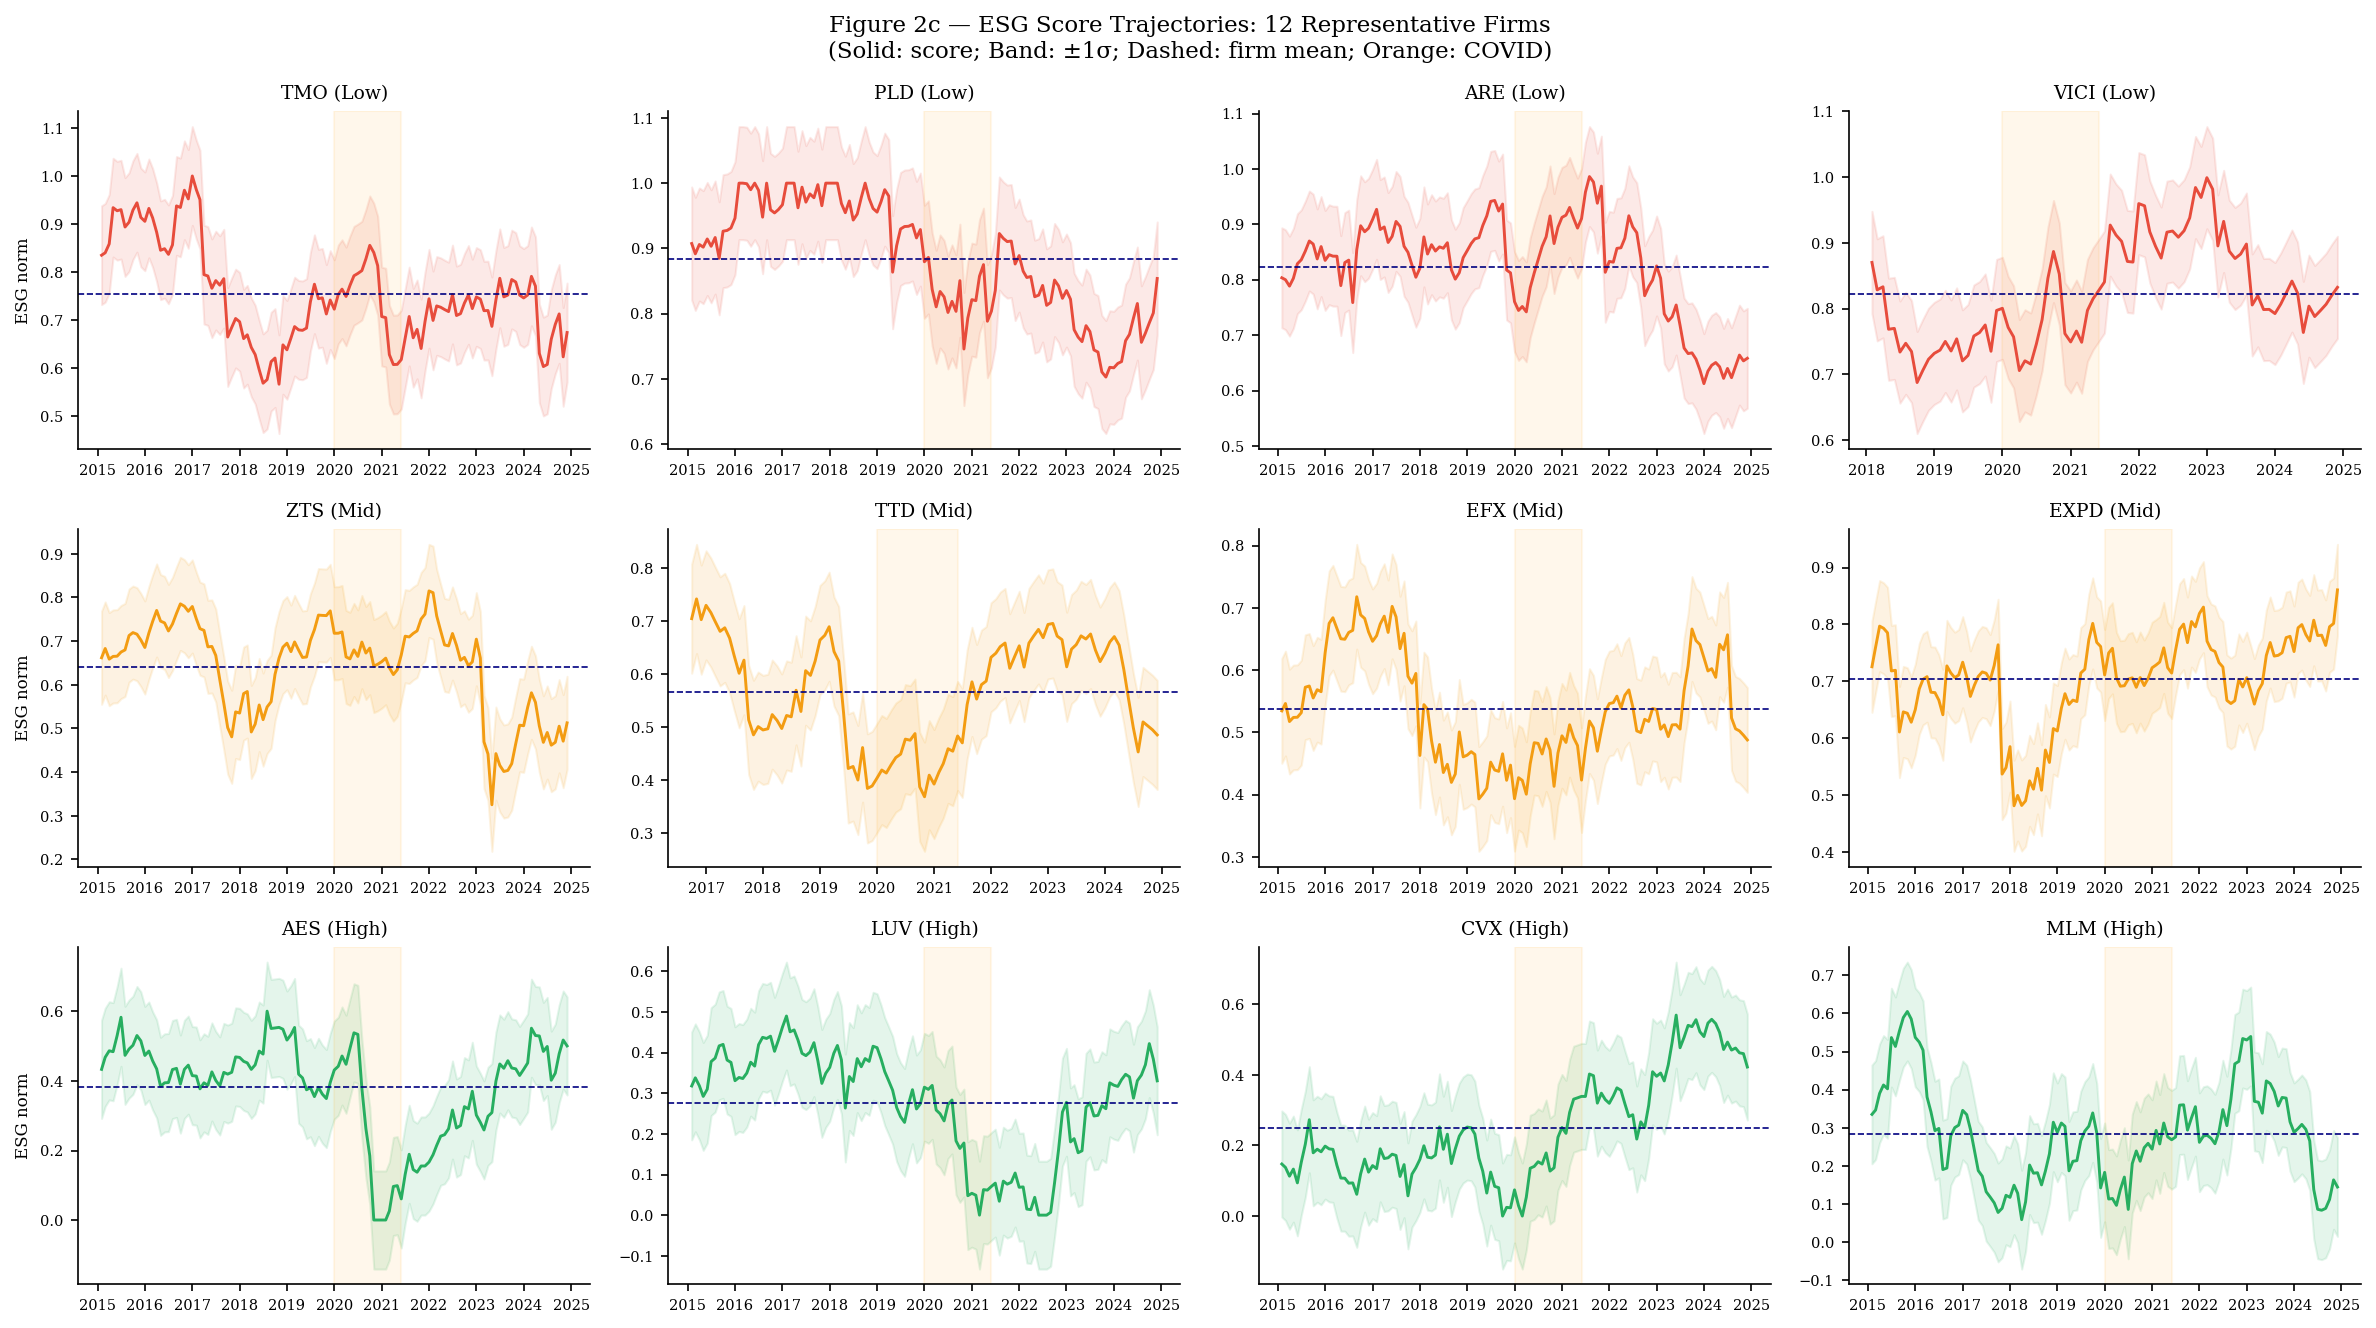
\includegraphics[width=\textwidth]{Pictures/fig2c_esg_trajectories.png}
  \caption{\textbf{Figure 2b --- Time-Varying ESG Score Trajectories.}
  Monthly normalised ESG score for twelve representative firms sampled across ESG terciles and GICS sectors. Solid line: score. Shaded band: $\pm 1\sigma$. Dashed line: firm mean. Orange shading: COVID-19 period (Jan 2020--Jun 2021). Within-firm variation is the identifying variation for M2 and M6.}
  \label{fig:esg_trajectories}
\end{figure}

The $\Delta\mathrm{ESG}$ distribution shown in Figure~\ref{fig:esg_distribution} is approximately symmetric around zero, ruling out directional interpolation bias.


%----------------------------------------------------
\section{Methodology}
%----------------------------------------------------

\subsection{Pre-Regression Diagnostic Pipeline}
\label{sec:diagnostics}

All model specification choices are driven by a pre-regression diagnostic pipeline rather than arbitrary convention. Table~\ref{tab:diagnostics} summarises the four tests and their implications.

\begin{table}[H]
  \centering
  \caption{Pre-Regression Diagnostic Tests. Tests are run on the full 56,656-observation panel prior to any hypothesis testing.}
  \label{tab:diagnostics}
  \small
  \begin{tabular}{l>{\raggedright\arraybackslash}p{3.0cm}cc>{\raggedright\arraybackslash}p{4.1cm}}
    \toprule
    & Test & Statistic & $p$-value & Implication \\
    \midrule
    D1 & Hausman (Mundlak)      & $\chi^2 = 12.044$ & $<0.001$ & FE preferred over RE \\
    D2 & Pesaran CD             & $129.867$         & $<0.001$ & Cross-sectional dependence present; clustered SEs used \\
    D3 & Wooldridge AR(1)       & $F = 87.194$      & $<0.001$ & Serial correlation present; Newey-West SEs applied \\
    D4 & VIF (M6 regressors)    & max VIF $= 1.075$ & ---      & Mean-centering $\Delta$ESG resolves collinearity \\
    \bottomrule
  \end{tabular}
  \smallskip\\
  \footnotesize \textit{Notes}: D1 rejects random effects in favour of fixed effects ($p<0.001$). D2 and D3 jointly justify both firm-clustered and Newey-West (12-lag) standard errors. D4 confirms that mean-centring $\Delta\mathrm{ESG}^c$ before interaction construction keeps all VIFs below the conventional threshold of 5.
\end{table}

\subsection{Panel Fixed Effects Regression}

All panel specifications include firm and year fixed effects, estimated by within-group demeaning. The Hausman test (D1) mathematically justifies fixed over random effects. Standard errors are clustered at the firm level (D2) and, where serial correlation is a concern, Newey-West with twelve lags is applied (D3). The first observation per firm is dropped in $\Delta\mathrm{ESG}$ specifications to avoid using returns without valid lagged ESG changes.

\subsection{Fama-MacBeth Cross-Sectional Regressions}

Each month $t$, excess returns are regressed cross-sectionally on full-period OLS beta and time-varying ESG level. The time series of monthly ESG slope coefficients is averaged and tested using Newey-West standard errors with twelve lags \citep{newey1987simple}, testing whether ESG level commands a cross-sectional risk premium independently of within-firm dynamics.


%========================================================
% CHAPTER 4: RESULTS
%========================================================
\chapter{Results}
\label{chap:results}

This chapter reports four empirical findings, each building on the last. The through-line is a single claim: ESG change, not ESG level, is the operative pricing variable. The four sections establish this sequentially --- first ruling out a static cross-sectional greenium, then documenting contemporaneous and predictive effects of $\Delta$ESG, and finally revealing the Beta Amplification Paradox. 

%----------------------------------------------------
\section{Full Hypothesis Test Table}
%----------------------------------------------------
 
\begin{table}[H]
  \centering
  \caption{Complete Hypothesis Test Summary. Bonferroni threshold: $\alpha/6 \approx 0.008$. BH-FDR at $q=0.05$.}
  \label{tab:hyp_full}
  \small
  \begin{tabular}{lllccccc}
    \toprule
    ID & Research Q & Model & Coeff & Raw $p$ & Bonf.\ $p$ & BH $p$ & Decision \\
    \midrule
    H1 & ESG level within-FE     & M2  & 0.014  & 0.0002 & 0.0012 & 0.0083 & Reject*** \\
    H2 & ESG level cross-section & FM  & 0.0045 & 0.2797 & 1.000  & 0.050  & F.t.r. \\
    H3 & $\Delta$ESG contemp.    & M6  & 0.0203 & 0.0167 & 0.1002 & 0.0333 & Reject** \\
    H4 & ESG momentum (FF5)      & P3  & 0.0243 & 0.0017 & 0.0102 & 0.0167 & Reject*** \\
    H5 & $\Delta$ESG$\times$Mkt  & M6  & 0.5304 & 0.0049 & 0.0294 & 0.0250 & Reject*** \\
    H6 & ESG level$\times$Mkt    & M2C & 0.1063 & 0.1492 & 0.8952 & 0.0417 & F.t.r. \\
    \bottomrule
  \end{tabular}
  \smallskip\\
  \footnotesize F.t.r.\ $=$ Fail to reject. H3--H5 survive BH-FDR at $q=0.05$; H1 and H4 survive Bonferroni.
\end{table}

%----------------------------------------------------
\section{ESG Level: No Cross-Sectional Greenium (H1, H2)}
\label{sec:level}
%----------------------------------------------------

\subsection*{Within-Firm Level Effect (H1)}

Model M2 regresses excess returns on market risk and the time-varying ESG level with entity and year fixed effects. The within-FE coefficient is $\hat{\beta}_2 = 0.0140$ (SE $= 0.0038$, $t = 3.691$, $p = 0.0002$), surviving Bonferroni correction ($p_{\text{Bonf}} = 0.0012$). In months where a firm's normalised ESG score is 0.10 above its own historical average, excess return is approximately 14 basis points higher, conditional on market risk. This is a within-firm signal --- it says that firms become more valuable to investors when they are above their own ESG baseline, regardless of where that baseline sits in the cross-section.

\begin{figure}[H]
  \centering
  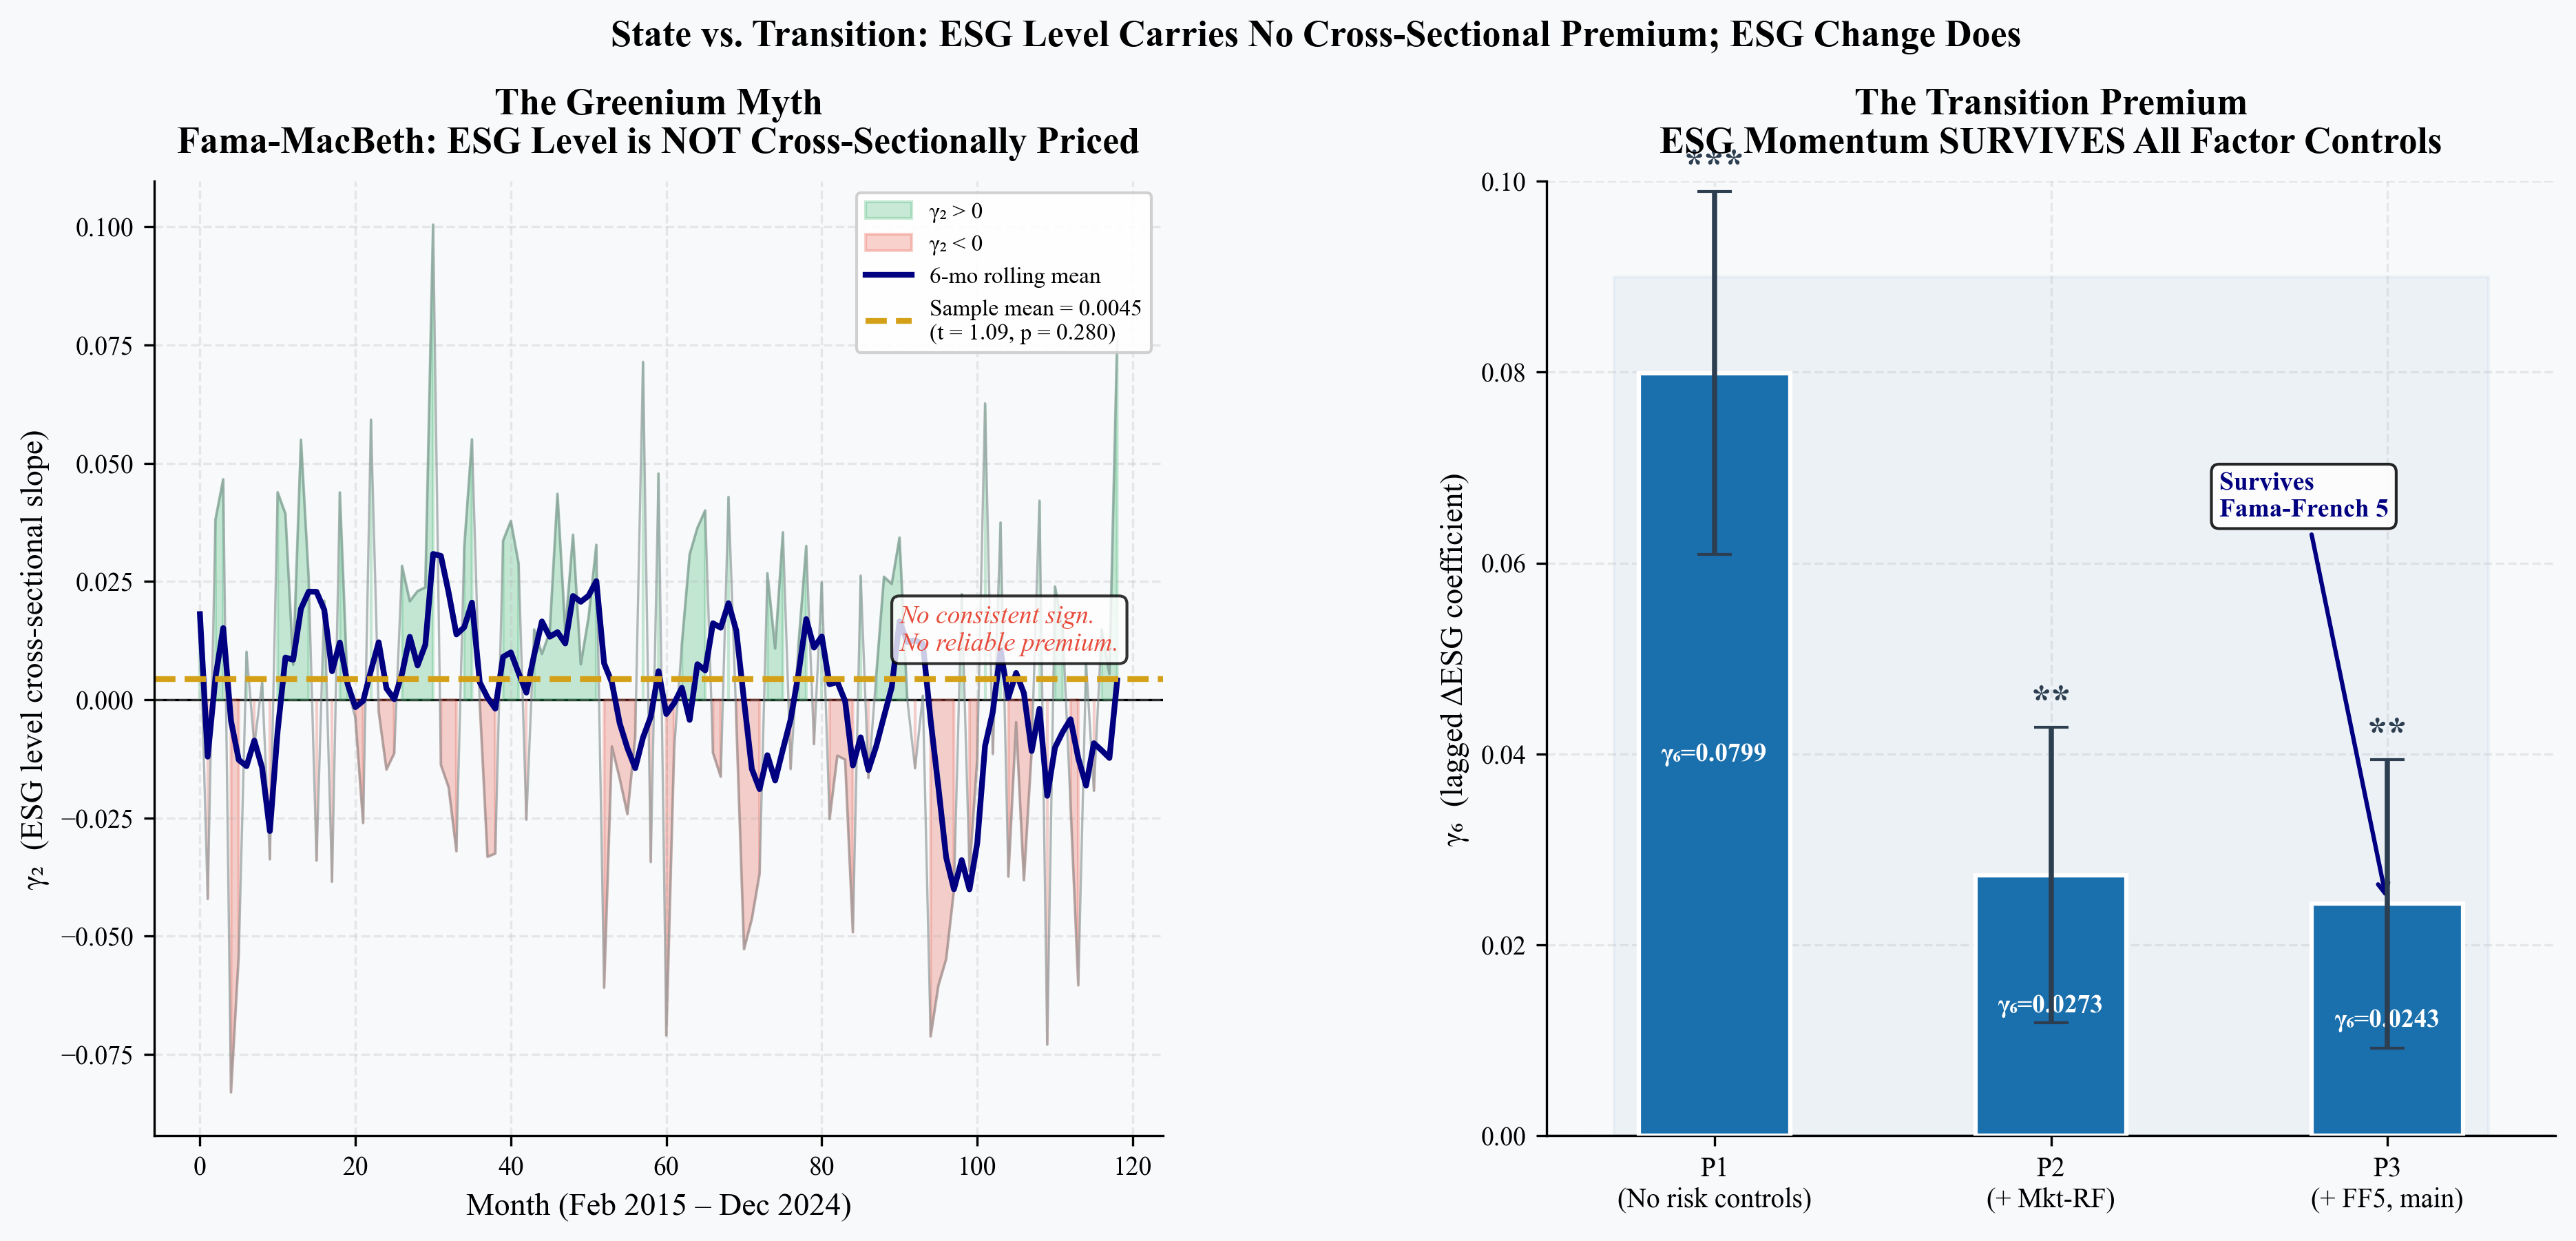
\includegraphics[width=\textwidth]{../Pictures/fig1_greenium_vs_transition.png}
  \caption{\textbf{Figure 5a --- Monthly ESG Coefficient (Fama-MacBeth) /  Monthly Cross-Sectional $R^2$.}
  Top: monthly cross-sectional ESG slope $\hat{\gamma}_{2,t}$; dashed line = full-sample mean. The irregular sign changes confirm that ESG level carries no persistent cross-sectional premium. Bottom: monthly $R^2$ across cross-sections.}
  \label{fig:fama_macbeth}
\end{figure}

\subsection*{No Cross-Sectional Premium (H2)}

The Fama-MacBeth test, however, tells a different story. Table~\ref{tab:fm} shows that the mean monthly ESG slope coefficient across 119 cross-sections is $\bar{\gamma}_2 = 0.00446$ with a Newey-West $t$-statistic of 1.086 ($p = 0.280$). ESG level does not command a reliable cross-sectional return premium. Figure~\ref{fig:fama_macbeth} confirms that the monthly ESG coefficient fluctuates in sign and magnitude throughout the sample, with no consistent direction.

\begin{table}[H]
  \centering
  \caption{Fama-MacBeth Cross-Sectional Regressions (H2). Mean slope coefficients with Newey-West standard errors (12 lags) across 119 monthly cross-sections. 479 firms.}
  \label{tab:fm}
  \begin{tabular}{lccccc}
    \toprule
    & $\bar{\gamma}$ & NW SE & $t$ & $p$ & Decision \\
    \midrule
    $\hat{\gamma}_0$ (intercept)   & 0.00110 & 0.00412 & 0.266 & 0.791 & --- \\
    $\hat{\gamma}_1$ (market beta) & 0.00864 & 0.00555 & 1.557 & 0.122 & F.t.r. \\
    $\hat{\gamma}_2$ (ESG level)   & 0.00446 & 0.00411 & 1.086 & \textbf{0.280} & F.t.r. \\
    \bottomrule
  \end{tabular}
  \smallskip\\
  \footnotesize F.t.r.\ $=$ Fail to reject. ESG$_{i,t}$ is time-varying normalised score; higher $=$ better ESG.
\end{table}



\noindent\textbf{Interpretation.} The divergence between H1 and H2 is itself a substantive finding. ESG level matters relative to a firm's own baseline (H1 rejects), but not as a cross-sectional characteristic separating high-ESG from low-ESG firms (H2 fails to reject). Static high ESG scores are already reflected in equilibrium prices. The return signal lives in the movement toward that score, not in the score itself.

%----------------------------------------------------
\section{ESG Changes Are Priced Contemporaneously (H3)}
\label{sec:change}
%----------------------------------------------------

\subsection*{The Aggregate Signal: Model M6}

Table~\ref{tab:panel} reports Models M1, M2, M2C, and M6 side by side. The key result is in M6: $\hat{\beta}_2 = 0.0203$ (SE $= 0.0085$, $t = 2.394$, $p = 0.017$). Within a given firm, a month in which the normalised ESG score improves by one unit above its mean is associated with a 2.03-percentage-point increase in excess return in that same month. This holds after conditioning on market risk, entity fixed effects, and year fixed effects. The economic mechanism is information flow: a rating revision signals changes in regulatory risk, governance quality, or operational sustainability that the market prices within the month. For large-cap S\&P 500 firms, rapid pricing is expected.

\subsection*{The Component-Level Failure: An Aggregate Synergy Signal}

When the composite $\Delta\mathrm{ESG}^c$ in M6 is replaced by the individual pillar changes $\Delta E^c$, $\Delta S^c$, and $\Delta G^c$ estimated separately, all three yield statistically insignificant coefficients: Environmental ($t = -0.201$, $p = 0.841$), Social ($t = 0.821$, $p = 0.411$), and Governance ($t$ not separately significant). The same pattern holds in the predictive specification (P3): $\Delta E^c$ ($t = -0.499$, $p = 0.618$), $\Delta S^c$ ($t = -0.565$, $p = 0.572$), $\Delta G^c$ ($t = -0.276$, $p = 0.782$) --- all insignificant.

This is a substantive finding. The market does not price changes to a firm's environmental footprint, its social practices, or its governance structure when considered in isolation. It prices the \emph{holistic composite}. Individual pillars carry too much idiosyncratic noise to move asset prices on their own; the Sustainalytics aggregate ESG score acts as a ``monolith'' rating that the market treats as a single, credible signal. This finding is consistent with the SASB materiality framework: what matters is the overall credibility of a firm's sustainability transition, not which specific dimension drives it.


\begin{table}[H]
  \centering
  \caption{Panel Fixed Effects Regressions (M1--M6). Dependent variable: monthly excess return. Entity and year FE. Standard errors clustered by firm.}
  \label{tab:panel}
  \begin{tabular}{lcccc}
    \toprule
    & M1 & M2 & M2C & M6 \\
    & CAPM & $+$ESG Level & $+$ESG$\times$Mkt & $+\Delta$ESG$\times$Mkt \\
    \midrule
    Mkt-RF                           & 0.9765*** & 0.9771*** & 0.9770*** & 0.9783*** \\
                                      & (0.0151)  & (0.0151)  & (0.0151)  & (0.0151)  \\[3pt]
    $\mathrm{ESG}_{i,t}$             &           & 0.0140*** &           &           \\
                                      &           & (0.0038)  &           &           \\[3pt]
    $\mathrm{ESG}_{i,t}^c$           &           &           & 0.0129*** &           \\
                                      &           &           & (0.0039)  &           \\[3pt]
    $\mathrm{ESG}_{i,t}^c\times$ Mkt-RF &        &           & 0.1063    &           \\
                                      &           &           & (0.0737)  &           \\[3pt]
    $\Delta\mathrm{ESG}_{i,t}^c$     &           &           &           & 0.0203**  \\
                                      &           &           &           & (0.0085)  \\[3pt]
    $\Delta\mathrm{ESG}_{i,t}^c\times$ Mkt-RF & &           &           & 0.5304*** \\
                                      &           &           &           & (0.1885)  \\[3pt]
    \midrule
    Entity FE                         & Yes & Yes & Yes & Yes \\
    Year FE                           & Yes & Yes & Yes & Yes \\
    $N$                               & 56,656 & 56,656 & 56,656 & 55,715 \\
    $R^2$                             & 0.2979 & 0.2980 & 0.2981 & 0.2991 \\
    Adj.\ $R^2$                       & 0.2917 & 0.2919 & 0.2920 & 0.2928 \\
    \bottomrule
  \end{tabular}
  \smallskip\\
  \footnotesize $^{***}p<0.01$, $^{**}p<0.05$, $^{*}p<0.10$. Superscript $c$ denotes mean-centred. M2C tests ESG-level beta modulation (H6: $t=1.442$, $p=0.149$, fails to reject). M6 tests $\Delta$ESG beta modulation (H5: $t=2.814$, $p=0.005$, rejects).
\end{table}


\noindent\textbf{Key message.} ESG improvements increase contemporaneous excess returns ($t=2.394$, $p=0.017$). Individual E, S, and G changes do not. The market prices the aggregate ESG change as an integrated information signal.

%----------------------------------------------------
\section[Lagged ESG Change Predicts Returns (H4)]{ESG Momentum: Lagged $\Delta$ESG Predicts Returns (H4)}
\label{sec:momentum}
%----------------------------------------------------

The predictive regressions P1--P3 test whether last month's ESG change forecasts this month's excess return. Table~\ref{tab:pred} shows results.

\begin{table}[H]
  \centering
  \caption{ESG Momentum: Predictive Regression Results (H4). Key variable: lagged $\Delta\mathrm{ESG}_{i,t-1}^c$. Entity and year FE. Firm-clustered SEs. $N=55{,}219$.}
  \label{tab:pred}
  \begin{tabular}{llccccc}
    \toprule
    Model & Controls & $\hat{\gamma}_6$ & SE & $t$ & $p$ & $R^2$ \\
    \midrule
    P1 & Entity + Year FE only & 0.0799 & 0.0097 & 8.251 & $<$0.001*** & 0.017 \\
    P2 & $+$ Mkt-RF            & 0.0273 & 0.0079 & 3.430 & 0.001***    & 0.301 \\
    P3 & $+$ FF5 (main)        & 0.0243 & 0.0077 & 3.140 & \textbf{0.002}*** & 0.306 \\
    \bottomrule
  \end{tabular}
  \smallskip\\
  \footnotesize $^{***}p<0.01$. P3 is the key specification: $\hat{\gamma}_6$ survives full Fama-French five-factor controls. The monotone attenuation from P1 to P3 confirms that part of the raw ESG predictability is absorbed by systematic risk factors, but a significant residual remains.
\end{table}

In P3, $\hat{\gamma}_6 = 0.0243$ ($t = 3.14$, $p = 0.002$), significant at the 1\% level and surviving Bonferroni correction ($p_{\text{Bonf}} = 0.010$). A firm that improved its ESG profile last month will --- all else equal --- earn higher excess returns this month even after market, size, value, profitability, and investment factors are controlled. Figure~\ref{fig:momentum} illustrates the economic magnitude: firms in the top quintile of lagged ESG improvement earn substantially higher next-month returns than those in the bottom quintile, with a near-monotone gradient.

\begin{figure}[H]
  \centering
  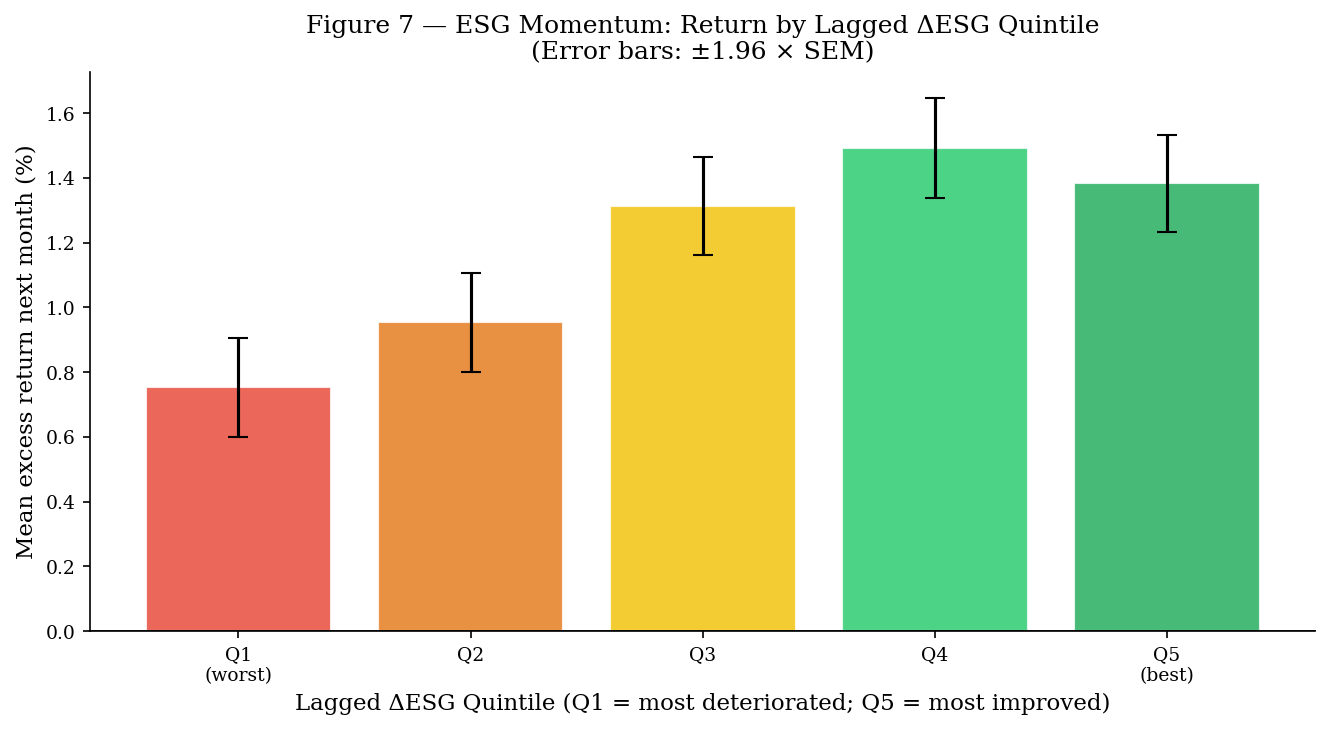
\includegraphics[width=0.82\textwidth]{../Pictures/fig7_esg_momentum.png}
  \caption{\textbf{Figure 5c --- ESG Momentum: Return by Lagged ESG Change Quintile.}
  Mean monthly excess return in the following period for firms sorted by quintile of lagged $\Delta\mathrm{ESG}_{i,t-1}^c$. Q1 = most deteriorated; Q5 = most improved. Error bars: $\pm1.96\times\mathrm{SEM}$. The monotone pattern confirms the ESG momentum channel documented in P1--P3.}
  \label{fig:momentum}
\end{figure}

The mechanism is gradual institutional rebalancing. ESG-screened mandates respond to score changes by adjusting holdings over multiple months due to position size constraints and mandate-driven rebalancing cycles. This creates a persistent demand shock that extends the price impact of an ESG improvement beyond the contemporaneous month, generating the predictability documented in P3.

\noindent\textbf{Key message.} ESG changes predict future returns ($t=3.14$, $p=0.002$). The market does not immediately and fully price ESG information: there is a momentum channel that generates exploitable next-month predictability net of five systematic risk factors.

%----------------------------------------------------
\section{The Beta Amplification Paradox (H5, H6)}
\label{sec:beta}
%----------------------------------------------------

\subsection*{$\Delta$ESG Amplifies Market Beta --- Not ESG Level}

The most original finding of this thesis concerns the interaction between ESG change and market risk. Returning to Table~\ref{tab:panel}, the interaction term in M6 is $\hat{\beta}_3 = 0.5304$ (SE $= 0.1885$, $t = 2.814$, $p = 0.005$). ESG improvements significantly \emph{amplify} market beta. A one-unit increase in $\Delta\mathrm{ESG}^c$ raises the firm's effective market beta loading by 0.5304 --- a substantial economic magnitude. This stands in sharp contrast to M2C, where the ESG-\emph{level}-by-market interaction is statistically insignificant ($t = 1.442$, $p = 0.149$, H6 fails to reject). It is the dynamic of ESG change, not the static level, that modulates systematic risk.

The direction is paradoxical relative to conventional expectations. The standard narrative holds that better-managed, more sustainable firms are less sensitive to macroeconomic shocks, and therefore carry lower betas. Our evidence shows the opposite: firms actively improving their ESG profile temporarily \emph{increase} their market co-movement. We term this the Beta Amplification Paradox and offer two complementary explanations.

\textbf{Transition risk.} Firms improving ESG are in operational transition --- investing in new sustainability infrastructure, restructuring supply chains, and absorbing governance changes. These activities are capital-intensive and operationally disruptive, increasing the firm's sensitivity to the macroeconomic environment during the transition period. A recession during an ESG transition amplifies losses; an expansion amplifies gains.

\textbf{Correlated institutional flows.} ESG improvements attract correlated inflows from ESG-screened institutional mandates. As multiple ESG funds simultaneously accumulate shares in an improving firm, the firm's return becomes more tightly coupled to the aggregate market through the common factor in institutional demand. This artificially increases beta during the inflow phase.



\subsection*{Sector Materiality: Where the ESG Signal Is Priced}

Table~\ref{tab:sector} and Figure~\ref{fig:forest} disaggregate the $\Delta$ESG contemporaneous return effect by GICS sector. The result confirms the SASB materiality hypothesis: the ESG change signal is priced where it is financially material and ignored where it is not.
In capital-intensive sectors --- Materials, Industrials, Consumer Discretionary, Financials --- an ESG improvement represents a genuine operational overhaul: a chemical plant reducing emissions, a manufacturer improving supply-chain governance, a bank restructuring lending criteria for ESG risk. These are material changes that directly alter regulatory exposure and enterprise risk, and the market prices them accordingly. In Information Technology ($p = 0.670$), by contrast, ESG improvements are frequently viewed as immaterial CSR activity with no bearing on the firm's fundamental value drivers, and the market does not price them.

\begin{table}[H]
  \centering
  \caption{$\Delta$ESG Return Effect by GICS Sector. Entity and year FE within-sector regressions. Key variable: $\Delta\mathrm{ESG}_{i,t}^c$.}
  \label{tab:sector}
  \begin{tabular}{lccccc}
    \toprule
    Sector & $N$ firms & $\hat{\beta}_{\Delta\mathrm{ESG}}$ & SE & $t$ & $p$ \\
    \midrule
    Materials              & 24 & 0.1153 & 0.0409 & 2.82 & 0.005*** \\
    Consumer Discretionary & 46 & 0.0719 & 0.0272 & 2.65 & 0.008*** \\
    Industrials            & 74 & 0.0577 & 0.0213 & 2.71 & 0.007*** \\
    Financials             & 74 & 0.0467 & 0.0160 & 2.91 & 0.004*** \\
    \midrule
    Energy                 & 21 & 0.0326 & 0.0370 & 0.88 & 0.379  \\
    Communication Services & 21 & 0.0229 & 0.0380 & 0.60 & 0.546  \\
    Information Technology & 67 & 0.0108 & 0.0254 & 0.43 & \textbf{0.670}  \\
    Real Estate            & 31 & 0.0078 & 0.0237 & 0.33 & 0.743  \\
    Health Care            & 56 & $-$0.0023 & 0.0274 & $-$0.08 & 0.934 \\
    Utilities              & 30 & $-$0.0140 & 0.0181 & $-$0.77 & 0.440 \\
    Consumer Staples       & 35 & $-$0.0453 & 0.0239 & $-$1.90 & 0.057* \\
    \bottomrule
  \end{tabular}
  \smallskip\\
  \footnotesize $^{***}p<0.01$, $^{**}p<0.05$, $^{*}p<0.10$. Top four sectors significant; bottom seven not significant at 5\%.
\end{table}

\subsection{ESG Momentum and Market Stress: A Regime-Dependent Perspective}

To further investigate the conditions under which ESG momentum is priced, we examine the relationship between ESG momentum and market stress over time. Specifically, we compute the 12-month rolling correlation between the ESG momentum spread (Q5–Q1 portfolio returns) and a proxy for market stress, measured using market volatility.

Figure \ref{fig:esg_stress_corr} presents the time-varying correlation alongside the corresponding evolution of market volatility and the ESG momentum spread. The correlation exhibits substantial temporal variation, ranging from strongly negative values (approximately $-0.6$) in the early sample period to strongly positive values (above $0.6$) in later years.

\begin{figure}[H]
    \centering
    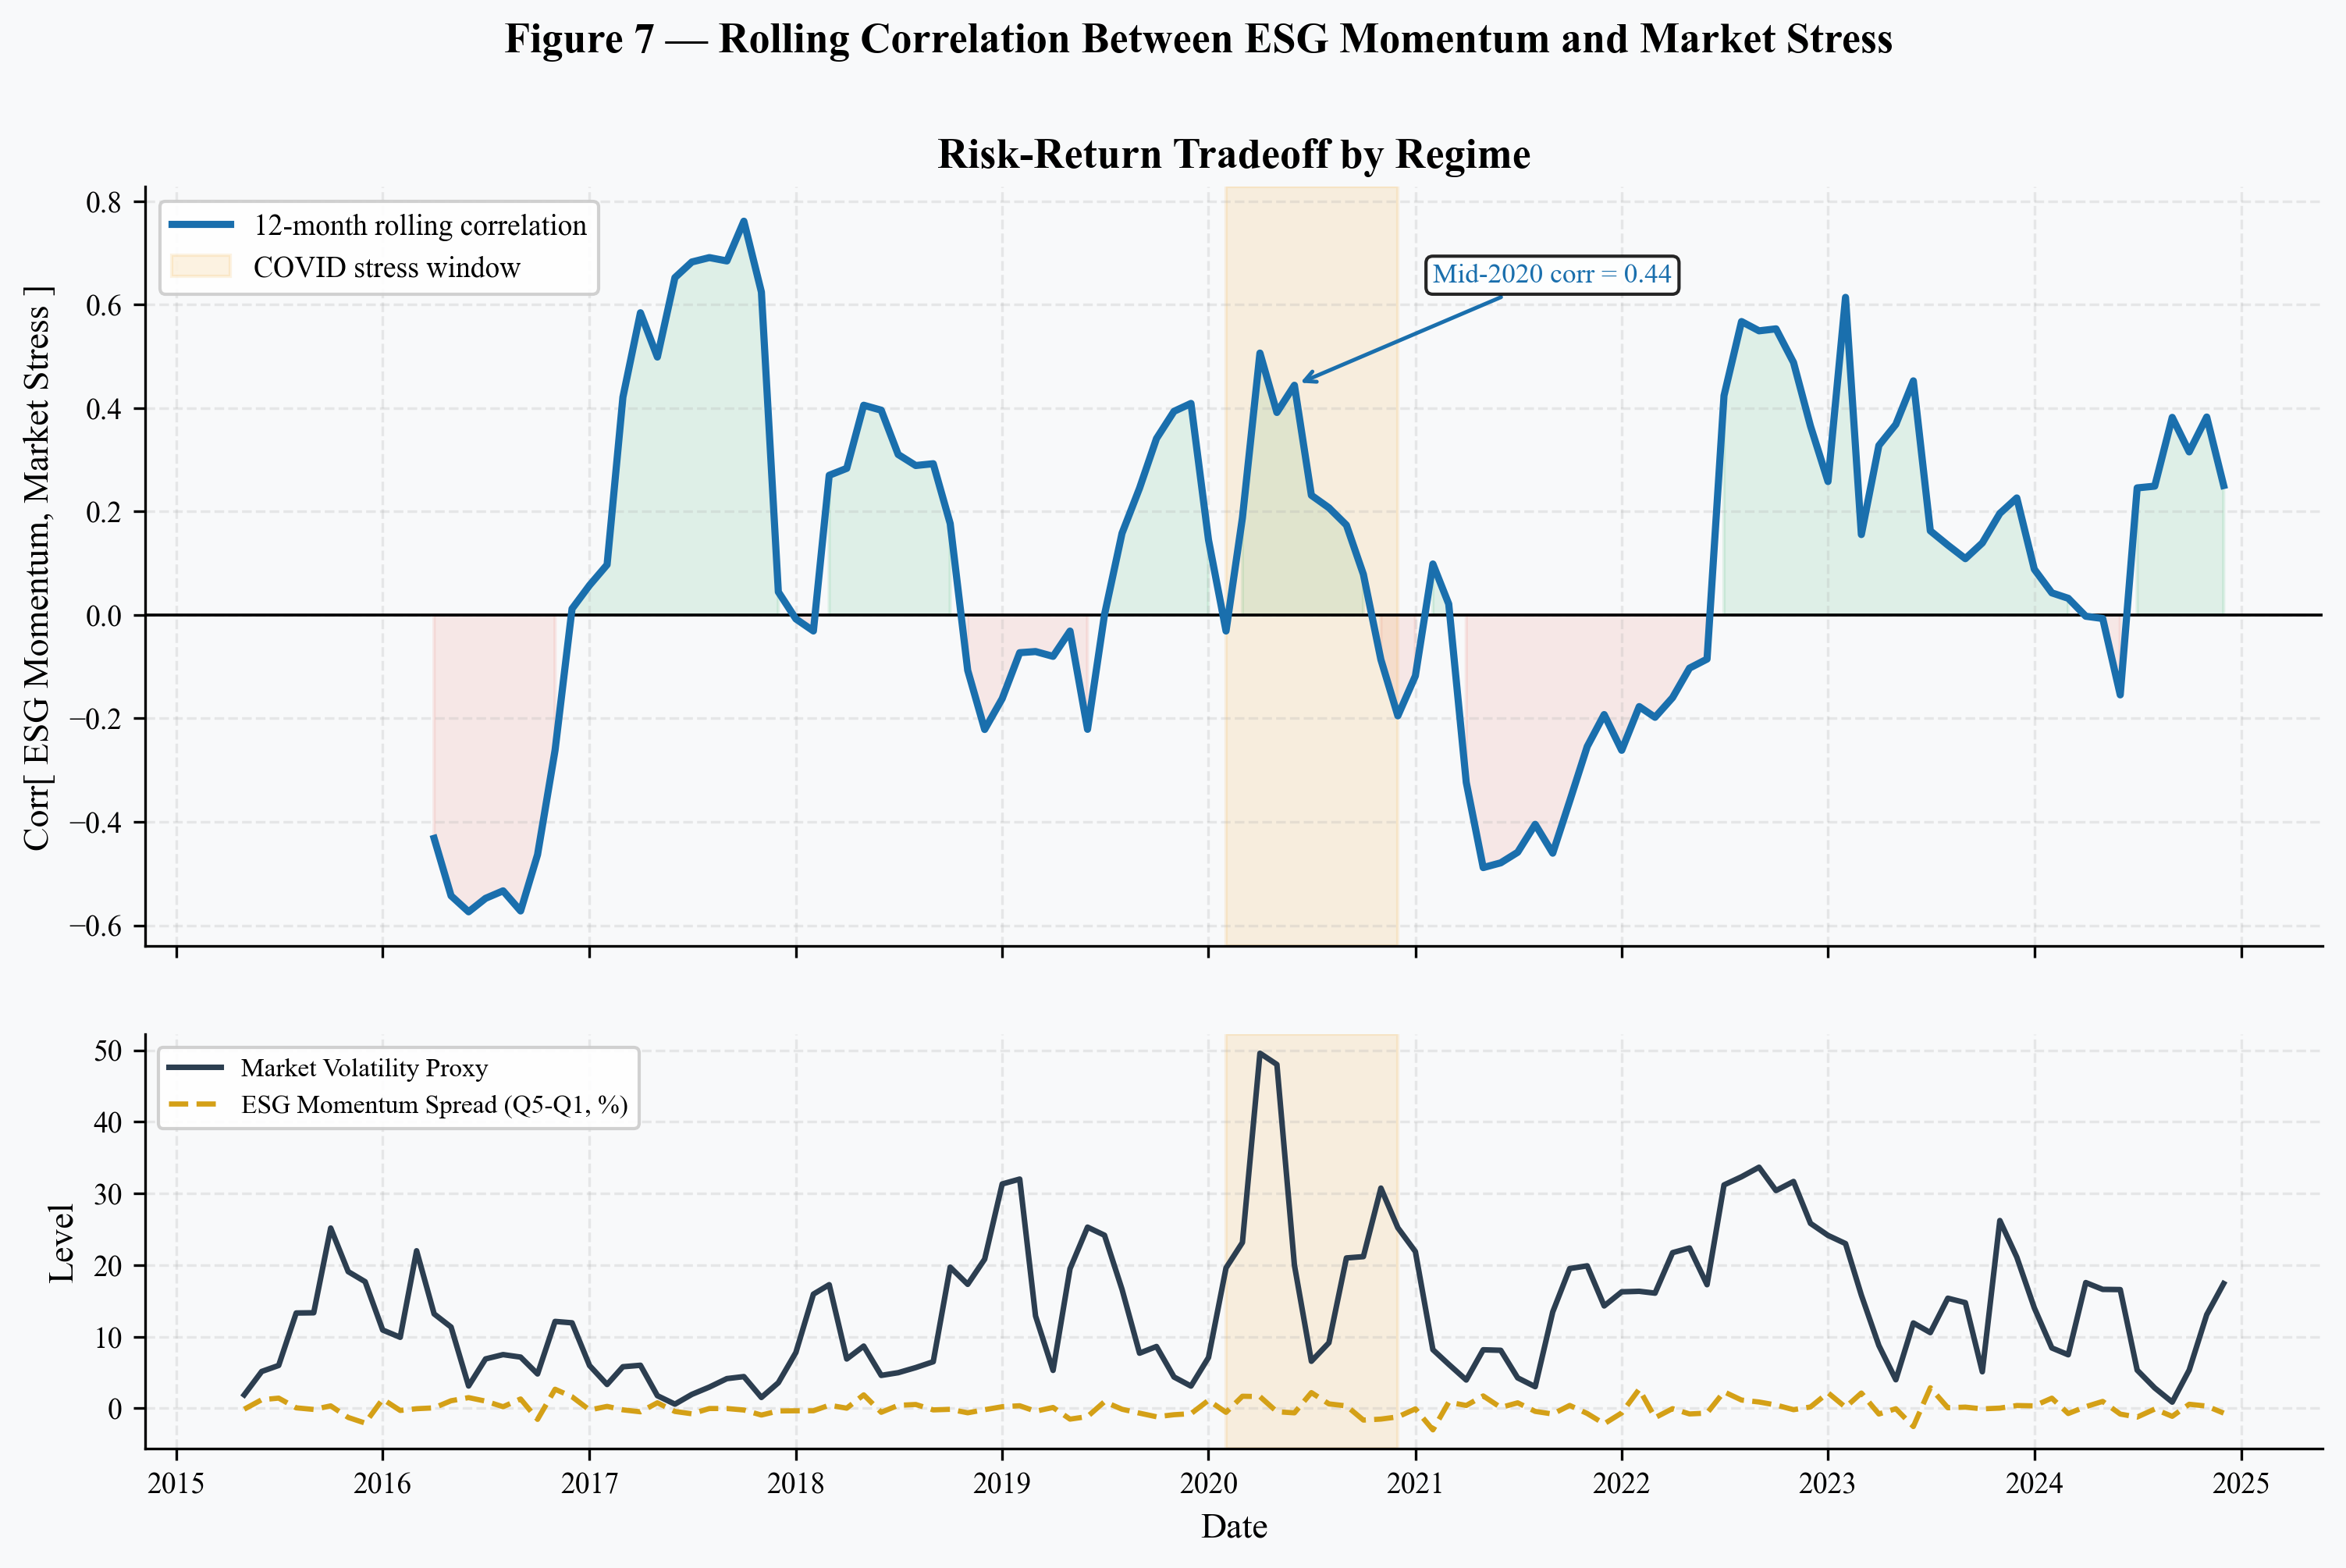
\includegraphics[width=0.9\linewidth]{../Pictures/fig7_regime_rolling_corr.png}
    \caption{Rolling Correlation Between ESG Momentum and Market Stress. 
    The top panel shows the 12-month rolling correlation between ESG momentum (Q5–Q1 spread) and a market volatility proxy. 
    The shaded region highlights the COVID-19 stress period (Jan 2020–Jun 2021). 
    The bottom panel displays the level of market volatility alongside the ESG momentum spread.}
    \label{fig:esg_stress_corr}
\end{figure}

A key observation emerges during the COVID-19 stress window. As market volatility spikes sharply, the rolling correlation turns significantly positive, reaching approximately $0.44$ at its peak. This indicates that ESG momentum strategies perform relatively better during periods of elevated market stress. In contrast, during calmer market conditions, the correlation weakens or turns negative, suggesting that ESG momentum is less consistently rewarded in low-volatility environments.

This evidence points to a regime-dependent structure in ESG pricing. ESG momentum does not behave as a static return factor; rather, its effectiveness depends critically on the prevailing market environment. During periods of heightened uncertainty, ESG improvements appear to act as a resilience signal, attracting capital flows toward firms perceived as more robust, better governed, or less exposed to downside risks.

The result complements the earlier findings on ESG momentum (H4) and the Beta Amplification Paradox (H5). While lagged ESG improvements generate statistically significant return predictability, the strength of this effect is conditional on market stress regimes. Taken together, the evidence suggests that ESG is best understood as a dynamic and state-dependent pricing factor, rather than a persistent cross-sectional premium.


%========================================================
% CHAPTER 5: DISCUSSION, LIMITATIONS, AND CONCLUSION
%========================================================
\chapter{Discussion, Limitations, and Conclusion}
\label{chap:discussion}

%----------------------------------------------------
\section{Discussion}
%----------------------------------------------------

The four results of Chapter~\ref{chap:results} cohere around a single interpretive frame: the market prices the \emph{transition process} of ESG improvement, not the \emph{state} of ESG attainment. This section elaborates on the three mechanisms that connect results to theory and addresses the paradox that is the thesis's most original contribution.

\textbf{Information flow and the transition narrative.} The contemporaneous pricing of $\Delta$ESG (H3: $t=2.394$, $p=0.017$) confirms that ESG rating revisions carry news. When Sustainalytics updates a firm's score, the revision aggregates information about recent operational changes, controversy resolutions, or governance improvements. This information is not perfectly anticipated by the market: the within-firm FE result (H1) shows that firms command a premium when they are above their own ESG baseline, consistent with the market updating its assessment of the firm's risk profile in real time as the score changes.

The shift from ``Does being green pay?'' to ``Does becoming green pay?'' resolves the apparent contradiction between H1 and H2. If high ESG scores are already reflected in equilibrium prices through sustained investor demand --- as the insignificant Fama-MacBeth result (H2: $p=0.280$) implies --- then there is no level premium to harvest. The exploitable signal is in the direction of ESG movement: firms becoming greener earn positive returns because the market updates their valuation as new information arrives, not because high-ESG firms as a class are systematically underpriced.

\textbf{Institutional rebalancing and the momentum channel.} The ESG momentum finding (H4: $t=3.14$, $p=0.002$) confirms that ESG information is not fully absorbed instantaneously. ESG-screened institutional mandates --- pension funds, ESG ETFs, and SRI funds --- respond to score upgrades by incrementally increasing their holdings over multiple months, constrained by position size limits, rebalancing cycles, and liquidity constraints. This creates a persistent demand shock that generates return predictability beyond the contemporaneous month. The result establishes $\Delta$ESG as a viable candidate for a factor-based investment strategy, complementing but distinct from classical price momentum \citep{jegadeesh1993returns}.

\textbf{The Beta Amplification Paradox and transition risk.} The finding that ESG improvements amplify market beta (H5: $\hat{\beta}_3=0.5304$, $t=2.814$, $p=0.005$) is the thesis's most original and counterintuitive contribution. The conventional ESG-risk narrative holds that better-managed, more sustainable firms are less exposed to systematic shocks. Our evidence shows the opposite holds \emph{during the transition period}.

Two mechanisms are at work simultaneously. First, ESG improvement is not free: it requires capital expenditure on sustainability infrastructure, operational restructuring, and potentially painful supply-chain adjustments. A firm in the middle of an ESG transition is more exposed to macroeconomic conditions than a firm that has completed one. Second, an ESG upgrade attracts correlated inflows from ESG-screened mandates: multiple institutional investors simultaneously accumulating the same stock increases its co-movement with the aggregate market through a common institutional demand factor. Both forces increase beta during the transition phase.

The sector-level evidence reinforces this interpretation. Materials, Industrials, Consumer Discretionary, and Financials --- the sectors where ESG improvements are SASB-material and involve genuine operational overhaul --- show significant $\Delta$ESG return effects. Information Technology ($p=0.670$), where ESG is frequently viewed as immaterial CSR, shows no effect. The market prices ESG transitions where they are real and ignores them where they are cosmetic.

%----------------------------------------------------
\section{Limitations}
%----------------------------------------------------

\textbf{Synthetic ESG panel.} The monthly ESG series is constructed via stochastic interpolation rather than directly observed monthly scores. Although the Ornstein-Uhlenbeck calibration preserves annual anchors and replicates empirical ESG autocorrelation, some within-year variation remains synthetic. The $\Delta$ESG coefficients are therefore likely a lower bound on the true ESG-change return relationship, and the reported effects may be attenuated by interpolation smoothness.

\textbf{Large-cap bias.} The sample is restricted to S\&P 500 firms. These are the most liquid, most analyst-covered, and most institutionally held equities in the U.S., meaning ESG information is incorporated relatively rapidly and institutional ESG flows represent a large fraction of trading volume. The ESG momentum effect may be substantially larger in the small-cap universe where information diffusion is slower and market microstructure is less efficient.

\textbf{U.S.-only data.} The analysis covers only U.S. equities. International markets differ substantially in ESG disclosure requirements, regulatory environments, and institutional investor ESG mandate penetration. The Beta Amplification Paradox and ESG momentum channel may operate with different magnitudes or signs in European markets, where mandatory ESG reporting under the SFDR has altered both the information environment and the institutional investor response function.

\textbf{Short effective horizon.} The ten-year sample (2015--2024) encompasses the pre-ESG-mainstream period and the surge in institutional ESG adoption, as well as the COVID-19 shock. The structural shift in institutional ESG mandates during this window makes it difficult to separate the ESG momentum premium from a secular shift in ESG demand. Longer samples with richer variation in ESG investor composition would strengthen causal identification.

%----------------------------------------------------
\section{Conclusion}
%----------------------------------------------------

This thesis reoriented the ESG-return question from state to transition. Rather than asking whether high-ESG firms earn higher returns --- a question that presupposes a static greenium that the Fama-MacBeth evidence consistently fails to confirm ($t=1.086$, $p=0.280$) --- it asked whether firms \emph{becoming} more sustainable earn higher returns. The answer across 56,656 firm-months of S\&P 500 data is unambiguous: yes, and through multiple reinforcing channels.

ESG improvements are priced contemporaneously ($\hat{\beta}=0.0203$, $t=2.394$, $p=0.017$), confirming rapid information incorporation. Lagged ESG improvements predict next-month returns after five-factor controls ($\hat{\gamma}=0.0243$, $t=3.14$, $p=0.002$), establishing an ESG momentum channel driven by gradual institutional rebalancing. And ESG improvements amplify rather than dampen market beta ($\hat{\beta}_{int}=0.5304$, $t=2.814$, $p=0.005$), revealing the Beta Amplification Paradox: firms in ESG transition are \emph{more} exposed to systematic risk, not less, during the transition period.

None of these effects can be detected using individual E, S, or G pillar changes. It is the holistic composite rating that the market treats as a credible signal. And the signal is concentrated in sectors where ESG is SASB-material --- Materials, Industrials, Consumer Discretionary, Financials --- and invisible in sectors like Information Technology where ESG changes are perceived as immaterial.

The implications run in two directions. For investors, an ESG momentum strategy --- tilting toward firms with recent aggregate ESG improvements in SASB-material sectors --- offers incremental return predictability beyond standard factor models, at the cost of temporarily elevated systematic risk during the transition period. For researchers, treating ESG as a static cross-sectional characteristic will continue to produce the mixed, inconclusive evidence that has frustrated the field. The dynamic dimension of ESG --- its changes, not its levels --- is where the asset pricing signal lives.
%\clearpage
\appendix
\section*{Appendix A: Code, Data, and Reproducibility}

To ensure full transparency and reproducibility of the empirical analysis presented in this thesis, all code, processed datasets, and supporting materials have been made publicly available in an online repository:

\begin{center}
\texttt{https://github.com/codegeek03/Does-Being-Green-Really-Pay-}
\end{center}

The repository is structured to reflect the complete research pipeline, from raw data ingestion to final result generation. The \texttt{src/analysis/} directory contains the core Python scripts used for data processing, model estimation, and visualization. In particular, the main script (\texttt{esg\_capm\_analysis.py}) implements the full empirical workflow, including panel construction, regression estimation, and hypothesis testing. Supplementary scripts generate publication-quality figures and additional robustness visualizations.

The \texttt{data/} directory is divided into raw and processed components. Raw data files include ESG scores, return series, and factor datasets obtained from external sources. These are transformed into a structured panel dataset stored in \texttt{data/processed/}, which serves as the primary input for all empirical models. Intermediate cleaning, normalization, and feature engineering steps are fully documented within the codebase.

All tables and figures reported in the thesis are reproducible through the scripts provided and are stored in the \texttt{results/} directory. This includes regression outputs, hypothesis test summaries, and graphical diagnostics. The repository also contains the complete \LaTeX{} source files for the thesis document in the \texttt{thesis/} folder, allowing for full replication of the written report.

A key component of the analysis is the construction of a high-frequency ESG panel using a stochastic interpolation framework. This is implemented in the script \texttt{stochastic\_esg\_simulator.py}, which models within-year ESG dynamics while preserving empirical properties such as persistence, sectoral co-movement, and event-driven shocks. This approach addresses the low-frequency nature of ESG disclosures and enables the estimation of time-varying effects.

To execute the analysis, users can run the main scripts from the repository root after installing the required Python dependencies. While the original development environment is not bundled, the code is modular and can be executed in any standard Python environment with commonly used data science libraries.

Overall, the repository is designed to provide a fully reproducible and extensible framework for studying ESG dynamics within asset pricing models. Researchers can adapt the pipeline to alternative datasets, extend the model specifications, or integrate additional factors for further analysis.

%----------------------------------------------------
%  BIBLIOGRAPHY
%----------------------------------------------------
\clearpage
\phantomsection
\addcontentsline{toc}{section}{Bibliography}
%\lhead{\emph{Bibliography}}
\nocite{*}
\bibliographystyle{plainnat}
\bibliography{Bibliography}

\end{document}